\documentclass[12pt, letterpaper]{article}
\title{Projet fin d'etude}
\author{COPIER 1\thanks{Funded by Achref aroua.}}
\date{2025}
\usepackage{graphicx}
\begin{document}
\maketitle
\newcounter{mainsection}  % Counter for the first number (1, 2, etc.)
\setcounter{mainsection}{1}  % Start from 1

\renewcommand{\thesection}{\arabic{mainsection}.\arabic{section}} % Format sections as X.Y




\newpage
\tableofcontents
\newpage

\listoffigures    % Table des figures
\newpage
\section*{Chapitre 1 }
\section{Introduction}
Ce chapitre comprend une présentation de l'entreprise \textbf{ALLOGENIE}, une présentation du projet avec le problème proposé et les solutions envisagées. Ce chapitre contient également une étude de deux sites web existants traitant du même sujet. Nous avons choisi une application principale, la plus utilisée. Ensuite, nous allons capturer les besoins fonctionnels de notre solution et enfin, nous présenterons la méthodologie utilisée pour notre projet.

\section{Présentation de l'entreprise}
\textbf{ALLOGENIE} est une startup canadienne qui se distingue par sa vision novatrice et son engagement à résoudre des problèmes sociaux et technologiques. L'entreprise repose sur des valeurs clés telles que l'innovation, la fiabilité et la qualité des services. ALLOGENIE utilise les nouvelles technologies pour proposer des solutions innovantes dans le domaine de l'ingénierie de développement et de l'intégration de solutions digitales adaptées aux besoins de ses utilisateurs.

ALLOGENIE valorise une approche centrée sur l'humain, ce qui lui permet de répondre efficacement aux attentes de ses clients tout en mettant en avant une expertise technique pointue. Sa structure à taille humaine permet d'exprimer pleinement des valeurs fondamentales, tout en offrant des services compétitifs à l'échelle nationale et internationale.



\section{Présentation du Projet}
\subsection{Problème}
Soumettre un CV à une entreprise peut souvent être un processus complexe et frustrant. Les candidats doivent adapter leur CV aux attentes des recruteurs, respecter des formats spécifiques, et naviguer sur différentes plateformes, ce qui peut entraîner des rejets liés à des incompatibilités ou à un manque de visibilité sur les critères requis. De l'autre côté, les recruteurs rencontrent également des difficultés à trouver des candidats qualifiés et à classer efficacement les CV reçus, ce qui prolonge les processus de recrutement et réduit leur efficacité.

Nous croyons en l'importance de simplifier ce processus pour les candidats comme pour les recruteurs, et nous travaillons à fournir des solutions adaptées à ces besoins.
\subsection{Solution}
Nous proposons une plateforme alimentée par l'intelligence artificielle qui permet aux utilisateurs de créer ou de soumettre leur CV facilement. La plateforme analyse les CV à l'aide de l'IA pour évaluer les qualifications des candidats par rapport aux offres d'emploi disponibles et informe les utilisateurs de leur niveau de correspondance avec chaque poste. 

Du côté des recruteurs, la plateforme offre un outil puissant pour identifier rapidement des candidats qualifiés répondant à leurs besoins. Notre solution est conçue pour être gratuite, conviviale, intuitive et sécurisée, facilitant ainsi le processus de recrutement tout en offrant une expérience utilisateur optimale pour les candidats.


ronnement plus flexible et accessible.
\section{\textbf{1.4 Étude des Solutions Existantes}}
\subsection{LinkedIn}
LinkedIn est une plateforme professionnelle largement utilisée qui permet aux utilisateurs de créer un profil détaillé, incluant leurs expériences professionnelles, leurs compétences, et leurs formations. Les recruteurs peuvent rechercher des candidats en fonction de critères spécifiques, et les utilisateurs peuvent postuler directement à des offres d'emploi.

\textbf{Avantages :}
\begin{itemize}
    \item Large base d'utilisateurs, ce qui augmente les chances de correspondance entre recruteurs et candidats.
    \item Possibilité de recommandations et de validation des compétences par d'autres utilisateurs.
    \item Intégration avec des outils de recrutement tiers.
\end{itemize}

\textbf{Limites :}
\begin{itemize}
    \item Complexité pour les nouveaux utilisateurs qui peuvent ne pas comprendre toutes les fonctionnalités.
    \item Les recruteurs doivent souvent payer pour des fonctionnalités avancées.
    \item Le tri des candidats peut manquer de précision pour certains besoins spécifiques.
\end{itemize}

\subsection{Indeed}
Indeed est un moteur de recherche d'emploi qui permet aux candidats de soumettre leur CV et de postuler à des milliers d'offres d'emploi en ligne. Les recruteurs peuvent publier des offres d'emploi et consulter des CV en ligne.

\textbf{Avantages :}
\begin{itemize}
    \item Facilité d'utilisation et interface intuitive pour les candidats et les recruteurs.
    \item Grand volume d'offres d'emploi disponibles.
    \item Accès gratuit pour les candidats.
\end{itemize}

\textbf{Limites :}
\begin{itemize}
    \item Le système de correspondance peut ne pas être suffisamment précis.
    \item Les candidats reçoivent souvent des recommandations d'emplois non pertinents.
    \item Difficulté à se démarquer pour les candidats en raison du grand nombre d'utilisateurs.
\end{itemize}
HEDHA BECH YETBADIL
\subsection{Réalité tunisienne}
Bien que les plateformes telles que LinkedIn et Indeed soient largement utilisées à l'international, en Tunisie, les outils spécialisés pour la gestion des CV et le recrutement restent limités. De nombreux candidats et recruteurs se tournent vers des groupes sur les réseaux sociaux, comme Facebook, pour trouver ou proposer des opportunités. 

\textbf{Problèmes de cette méthode :}
\begin{itemize}
    \item Absence de standardisation et de critères clairs pour évaluer les candidats.
    \item Risques de sécurité et de confidentialité des données.
    \item Difficulté à vérifier la fiabilité des candidats ou des recruteurs.
\end{itemize}

\subsection{Solution Proposée}
Notre solution consiste à développer une plateforme gratuite et conviviale pour répondre aux besoins des candidats et des recruteurs. Voici les principales fonctionnalités envisagées :
\begin{itemize}
    \item Création et soumission facile de CV.
    \item Analyse des CV à l'aide de l'intelligence artificielle pour évaluer les correspondances avec les offres d'emploi.
    \item Interface intuitive et sécurisée pour les utilisateurs.
    \item Recherche avancée pour permettre aux recruteurs de trouver rapidement des candidats qualifiés.
    \item Communication directe entre candidats et recruteurs via la plateforme.
    \item Vérification des profils pour garantir la fiabilité des utilisateurs.
\end{itemize}

\section{1.5 Méthodologie Utilisée}

\subsection{1.5.1 Approche de gestion de projet}
Dans notre projet, nous avons opté pour l'approche agile afin de gérer l'ensemble du projet. Nous avons choisi cette approche car les spécifications incluent des besoins qui ne sont pas très détaillés ni clairs. Nous avons également prévu que les besoins évolueront au fil du temps, comme cela est déjà mentionné dans les spécifications. 

Tous ces indicateurs nous ont amenés à choisir une approche agile pour gérer le projet, d'une part pour réussir à implémenter un maximum des fonctionnalités demandées, et d'autre part pour réussir à résister aux changements et aux nouveaux besoins. 

Une approche agile peut également nous faire gagner du temps en évitant le piège de l'effet tunnel, qui est l'un des inconvénients les plus connus et les plus graves d'une approche classique de gestion de projet. 

L'agilité est une approche itérative de gestion de projet et de développement logiciel qui aide les équipes à livrer de la valeur à leurs clients plus rapidement et avec moins de tracas. Au lieu de miser sur un lancement  big bang , une équipe agile livre du travail en petites tranches consommables. 

L'approche agile est caractérisée par sa flexibilité et son adaptabilité, contrairement aux approches traditionnelles de gestion de projet. Les méthodes agiles impliquent le demandeur (client) autant que possible et permettent une grande réactivité à ses demandes. 

Les concepts et outils agiles proviennent de l'informatique, mais les pratiques agiles sont désormais disponibles pour tous les métiers : des services innovants à la RD dans les industries lourdes. 

Il existe plusieurs méthodes agiles, notamment : Scrum, XP, RAD et DSDM.

\subsection{Présentation du cadre utilisé}
Nous avons défini les caractéristiques des méthodes agiles. Une étude des caractéristiques des méthodes agiles les plus utilisées nous a conduit à choisir la méthode Scrum. En effet, Scrum indique que la taille de l'équipe peut être réduite et c'est notre cas. Une autre raison est que Scrum est flexible en termes de durée de sprint (entre 2 et 4 semaines).

Scrum est un cadre de travail qui aide les équipes à collaborer. Tout comme une équipe de rugby (d'où il tire son nom) qui s'entraîne pour un grand match, Scrum encourage les équipes à apprendre par l'expérience, à s'auto-organiser lorsqu'elles travaillent sur un problème et à réfléchir à leurs victoires et à leurs échecs pour s'améliorer en continu.

Scrum appartient à la famille des méthodologies itératives et incrémentales et repose sur les principes et valeurs agiles. La plupart du temps, les experts Scrum, voire ses fondateurs, le décrivent comme un cadre ou un modèle orienté vers la gestion de projet qui peut intégrer différentes méthodes ou pratiques d'ingénierie.

\section{ Présentation et application de Scrum}
Dans cette partie, nous présenterons le backlog produit et la liste des acteurs impliqués dans notre projet.

Le cadre Scrum consiste à définir un cadre de travail permettant la réalisation de projets complexes. Les projets qui suivent la méthode agile Scrum sont divisés en plusieurs cycles de travail relativement courts appelés  sprints . Ceux-ci permettent aux membres de l'équipe de mieux planifier les prochaines étapes de développement du projet, mais aussi d'évaluer régulièrement les progrès réalisés par rapport au projet. Les sprints peuvent durer d'une à quatre semaines. Ils permettent également de réajuster ou de réorienter la direction prise par le projet si besoin.

En effet, la méthode Scrum présente plusieurs avantages en dehors de l'amélioration de la productivité et de la communication au sein du projet. Elle repose avant tout sur des rôles fixes, des responsabilités et des réunions qui ne changent jamais, tout en garantissant une gestion flexible et adaptative des projets. Cela a l'avantage de rassurer les équipes lors de certaines phases de développement.

\subsection{Liste des acteurs}
L'approche Scrum nécessite une équipe projet composée de plusieurs acteurs, chacun ayant un rôle bien défini. Dans notre cas, le rôle de Product Owner a été attribué à M. Oussama Bejaoui (superviseur professionnel). Le Product Owner exprime les besoins du client et fixe les délais de livraison des livrables. Le rôle de développeur a été confié à Mme Ilef Kaabi et Mme Ferdaous Ben Dhafer. Le développeur participe aux réunions quotidiennes Scrum en rapportant les tâches prévues pour chaque jour, assure au Product Owner et au Scrum Master que le travail alloué est effectué comme prévu, et veille à une compréhension claire des épics et des personas. Enfin, le rôle de Scrum Master a été attribué à M. Oussama Bejaoui (superviseur professionnel). Le Scrum Master est le leader d'une équipe qui applique Scrum. L'équipe de développement, composée de nous-mêmes, est responsable de transformer les besoins du client en un produit fonctionnel livré à temps.

\subsection{ Artifact réalisé par Scrum}
Ceci est l'un des artefacts de la méthode Scrum. L'équipe de développement doit s'accorder sur les conditions pour que les tâches et les histoires passent à l'état terminé. En ce sens, nous avons convenu en collaboration avec





\newpage
\stepcounter{mainsection} % Increment main section to 2
\setcounter{section}{0} 

\section*{Chapitre 2}
 \section*{Sprint 0 : Implementation de projet}
\subsection*{Introduction}
Décris ici les objectifs initiaux, l'analyse du projet, et la mise en place de l'environnement.

\section{Backlog de produit}
\begin{figure}[h]
    \centering
 

    \centering
    \includegraphics[width=0.8\textwidth]{Diagrams/backlog_finale.png}



    \caption{Backlog}
    \label{fig:Backlog}
\end{figure}
\maketitle

\section{Environnement et choix technologiques}

Les bons choix  outils pour notre travail est une étape cruciale pour rendre notre projet plus simple et efficace.

Dans cette section, on va vous parler des outils et des technologies que nous allons utiliser.

\subsection{Environnement}

Dans cette section, nous citons les diff\'erents outils utilis\'es pour la r\'ealisation de ce projet.


\section*{VS Code}
VS Code est un environnement de developpement integr\'e (IDE) populaire, offrant une prise en charge compl\`ete pour le d'eveloppement web et backend.\
 
\includegraphics[width=0.6\textwidth]{Logo/vs.png}

\textbf{Figure 2.3 – Logo de VS Code}
\subsubsection*{Postman}
Tailwind CSS est un framework CSS utilitaire permettant une conception rapide et efficace des interfaces utilisateur.\

 
\includegraphics[width=0.6\textwidth]{Logo/postman.png}

\textbf{Figure 2.9 – Logo de Tailwind CSS}
\subsubsection*{GitLab}
GitLab est une plateforme en ligne d'h'ebrgement de projets de d'eveloppement logiciel, utilisant Git comme syst\`eme de gestion de versions.\
\textbf{Figure 2.4 – Logo de GitLab}

\subsubsection*{StartUML}
StarUML est un outil UML permettant de cr'eer des diagrammes bien structur'es pour mod'eliser nos applications.\

 	
\includegraphics[width=0.6\textwidth]{  Logo/uml.png}

\textbf{Figure 2.5 – Logo de StarUML}

\subsubsection*{Name.com}
Name.com est une plateforme permettant l'achat et la gestion de noms de domaine pour nos applications.\
\textbf{Figure 2.6 – Logo de Name.com}

\subsubsection*{Notion}
Notion est un outil d'organisation et de gestion de projet, facilitant la collaboration et le suivi des t\^aches.\

 
\includegraphics[width=0.6\textwidth]{Logo/notion.jpg}

\textbf{Figure 2.7 – Logo de Notion}

\section{Pr'esentation des technologies utilis'ees}

\subsubsection*{React.js avec Vite}
React.js est une biblioth\`eque JavaScript pour la construction d'interfaces utilisateur dynamiques. Nous utilisons Vite comme outil de build rapide et efficace.\

 
\includegraphics[width=0.6\textwidth]{Logo/react.png}
 
\includegraphics[width=0.6\textwidth]{Logo/vite.png}
    \label{fig:reactlogo}

\textbf{Figure 2.8 – Logo de React.js}

\subsubsection*{Tailwind CSS}
Tailwind CSS est un framework CSS utilitaire permettant une conception rapide et efficace des interfaces utilisateur.\



\textbf{Figure 2.9 – Logo de Tailwind CSS}

\subsubsection*{Express.js}
Express.js est un framework minimaliste et flexible pour Node.js, facilitant le d'eveloppement d'API robustes.\

 
\includegraphics[width=0.6\textwidth]{Logo/express.jpg}

\textbf{Figure 2.10 – Logo d'Express.js}

\subsubsection*{MongoDB Atlas}
MongoDB Atlas est une base de donn'ees NoSQL g'er'ee dans le cloud, offrant une scalabilit'e et une s'ecurit'e accrues.\
\begin{figure}[h] 
 \centering
 
\includegraphics[width=0.6\textwidth]{Logo/mongodb.jpg}
 \caption{mongodb}
    \label{fig:mongodb}

\end{figure}


\subsubsection*{JWT (JSON Web Token)}
JSON Web Token (JWT) est une norme ouverte permettant la transmission s'ecuris'ee d’informations entre plusieurs parties sous forme d’objet JSON. Nous utilisons JWT pour l’authentification et le hachage des mots de passe pour garantir la s'ecurit'e des utilisateurs.\
\begin{figure}[h] 
 \centering
 
\includegraphics[width=0.6\textwidth]{Logo/jwt.jpg}
 \caption{JWT}
    \label{fig:JWT}
\end{figure}

\newpage
\section{Scenario complete d'application}
\subsection{BPMN}
\begin{figure}[h]
    \centering
    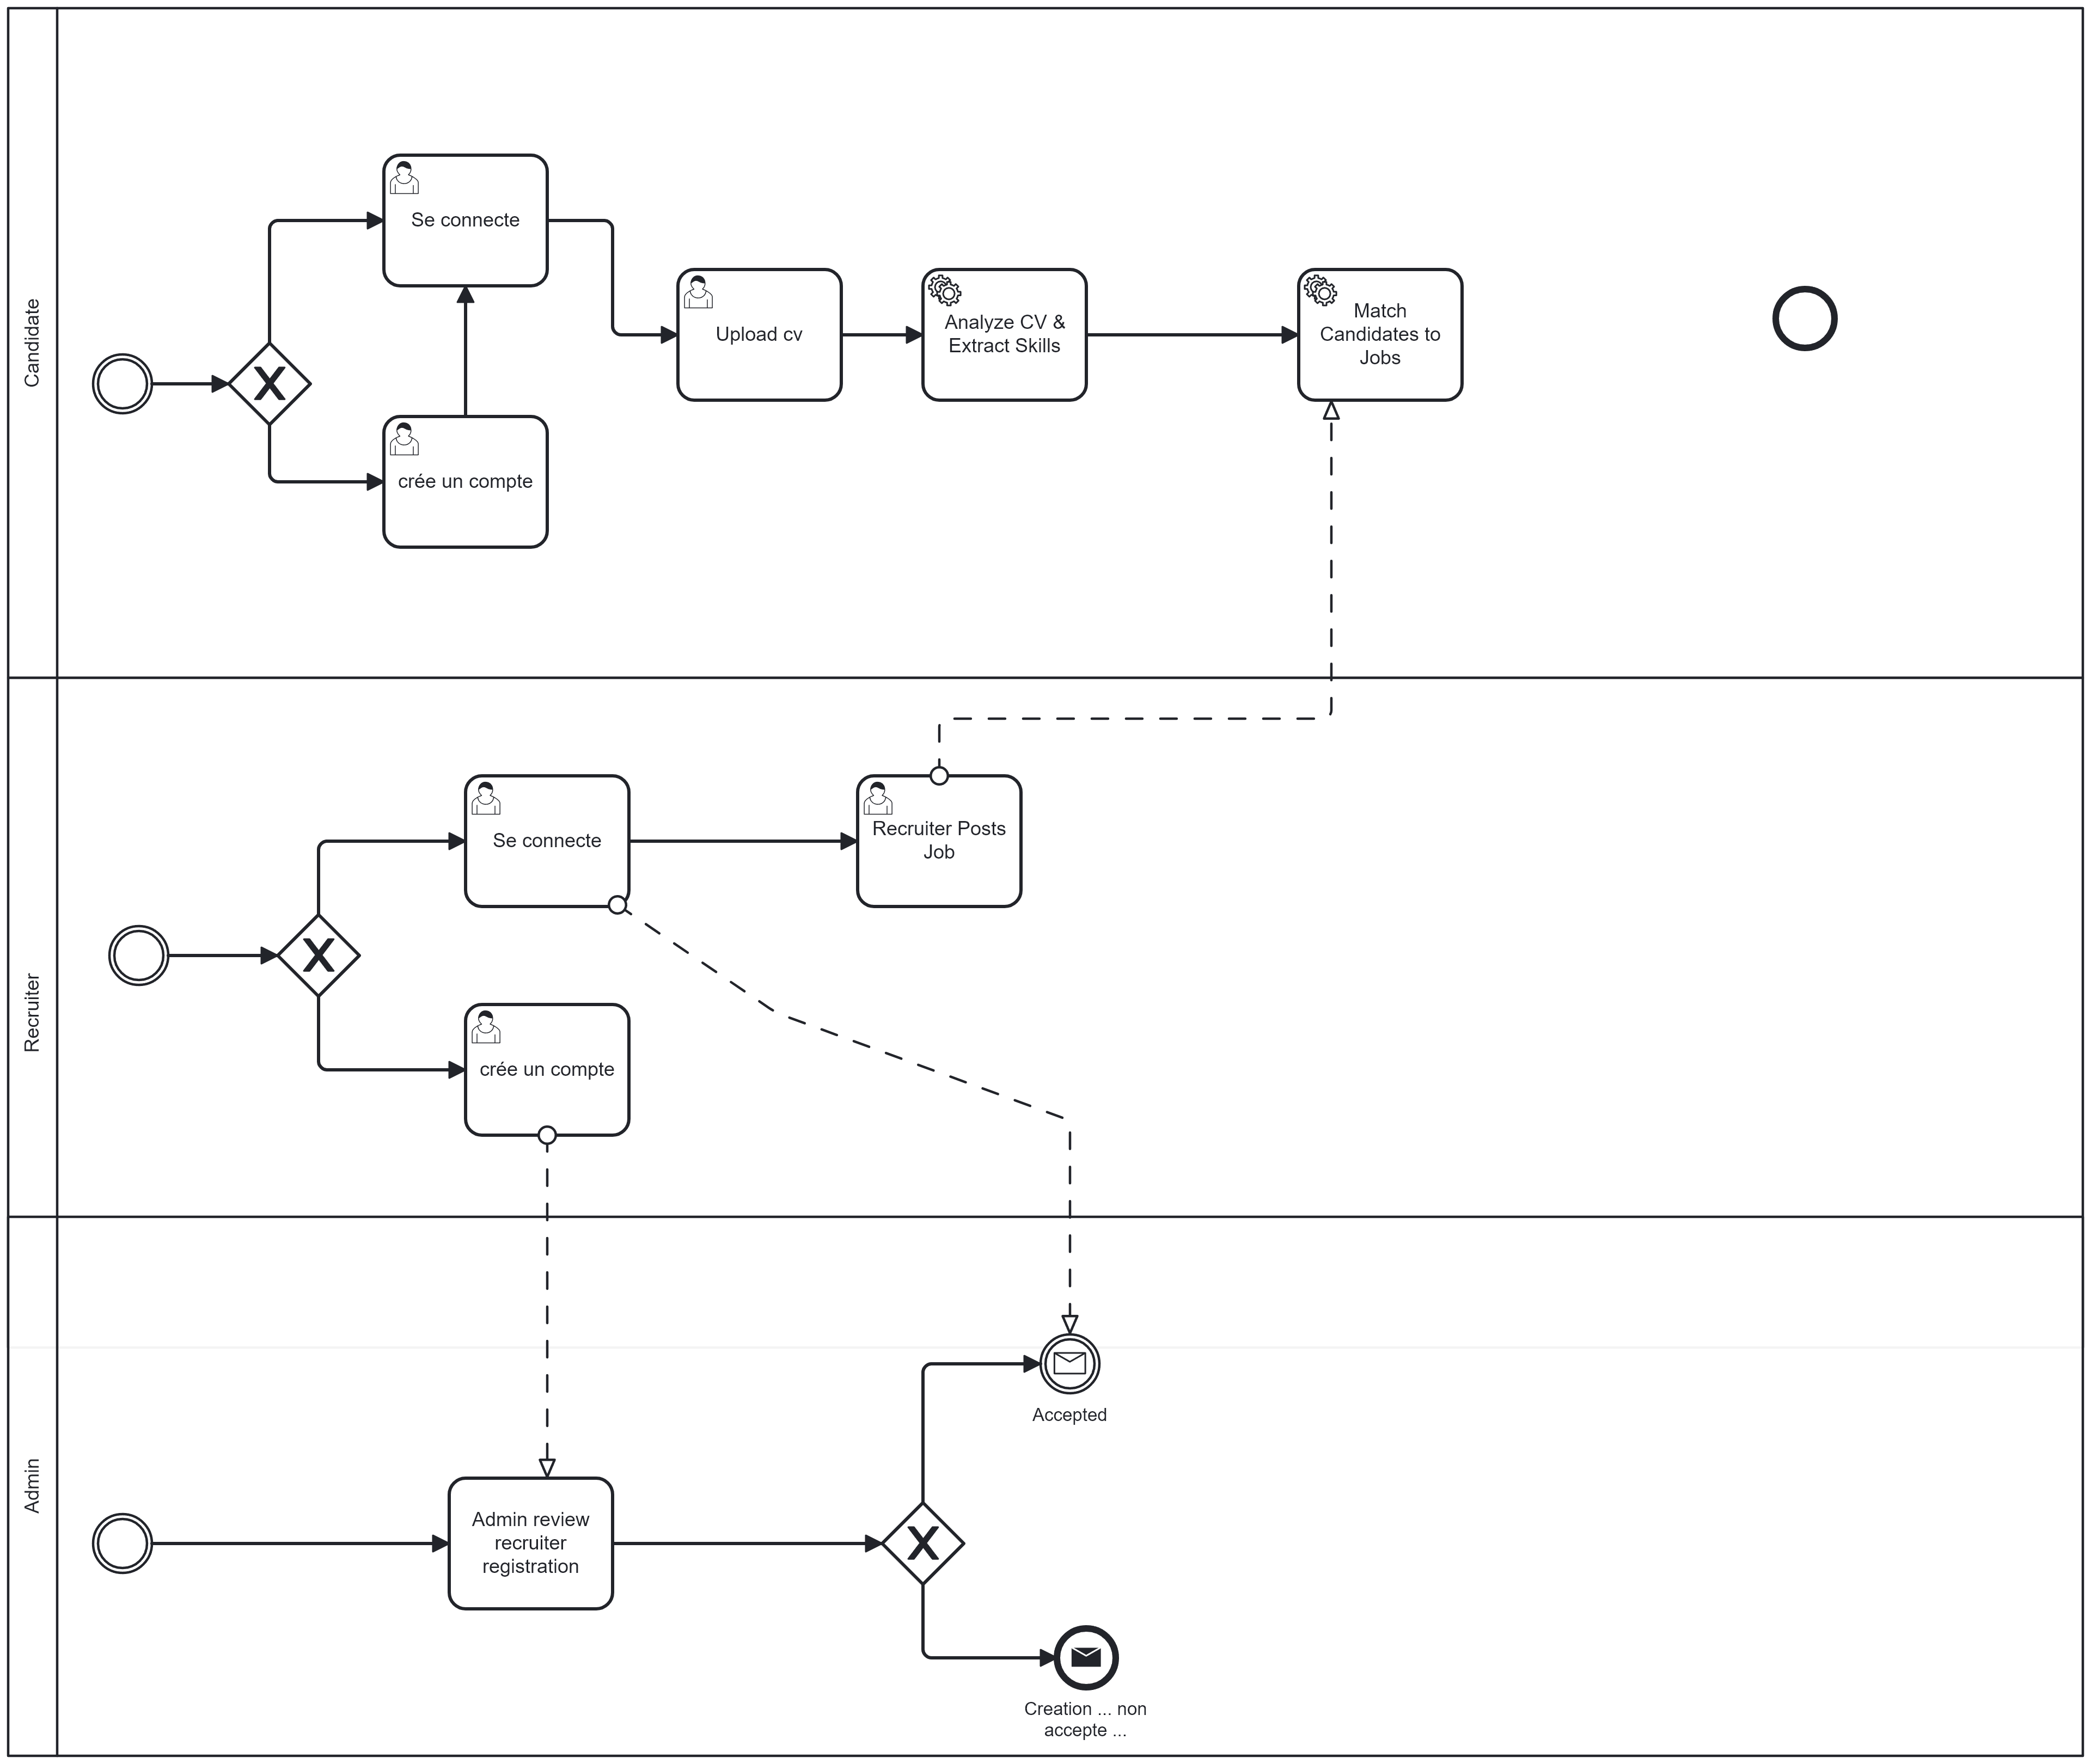
\includegraphics[width=0.9\textwidth]{Diagrams/BPMN_V1.png}
    \caption{BPMN}
    \label{fig:BPMN}
\end{figure}

\newpage
\subsection{Diagram d'ativité}
\begin{figure}[h]
    \centering
    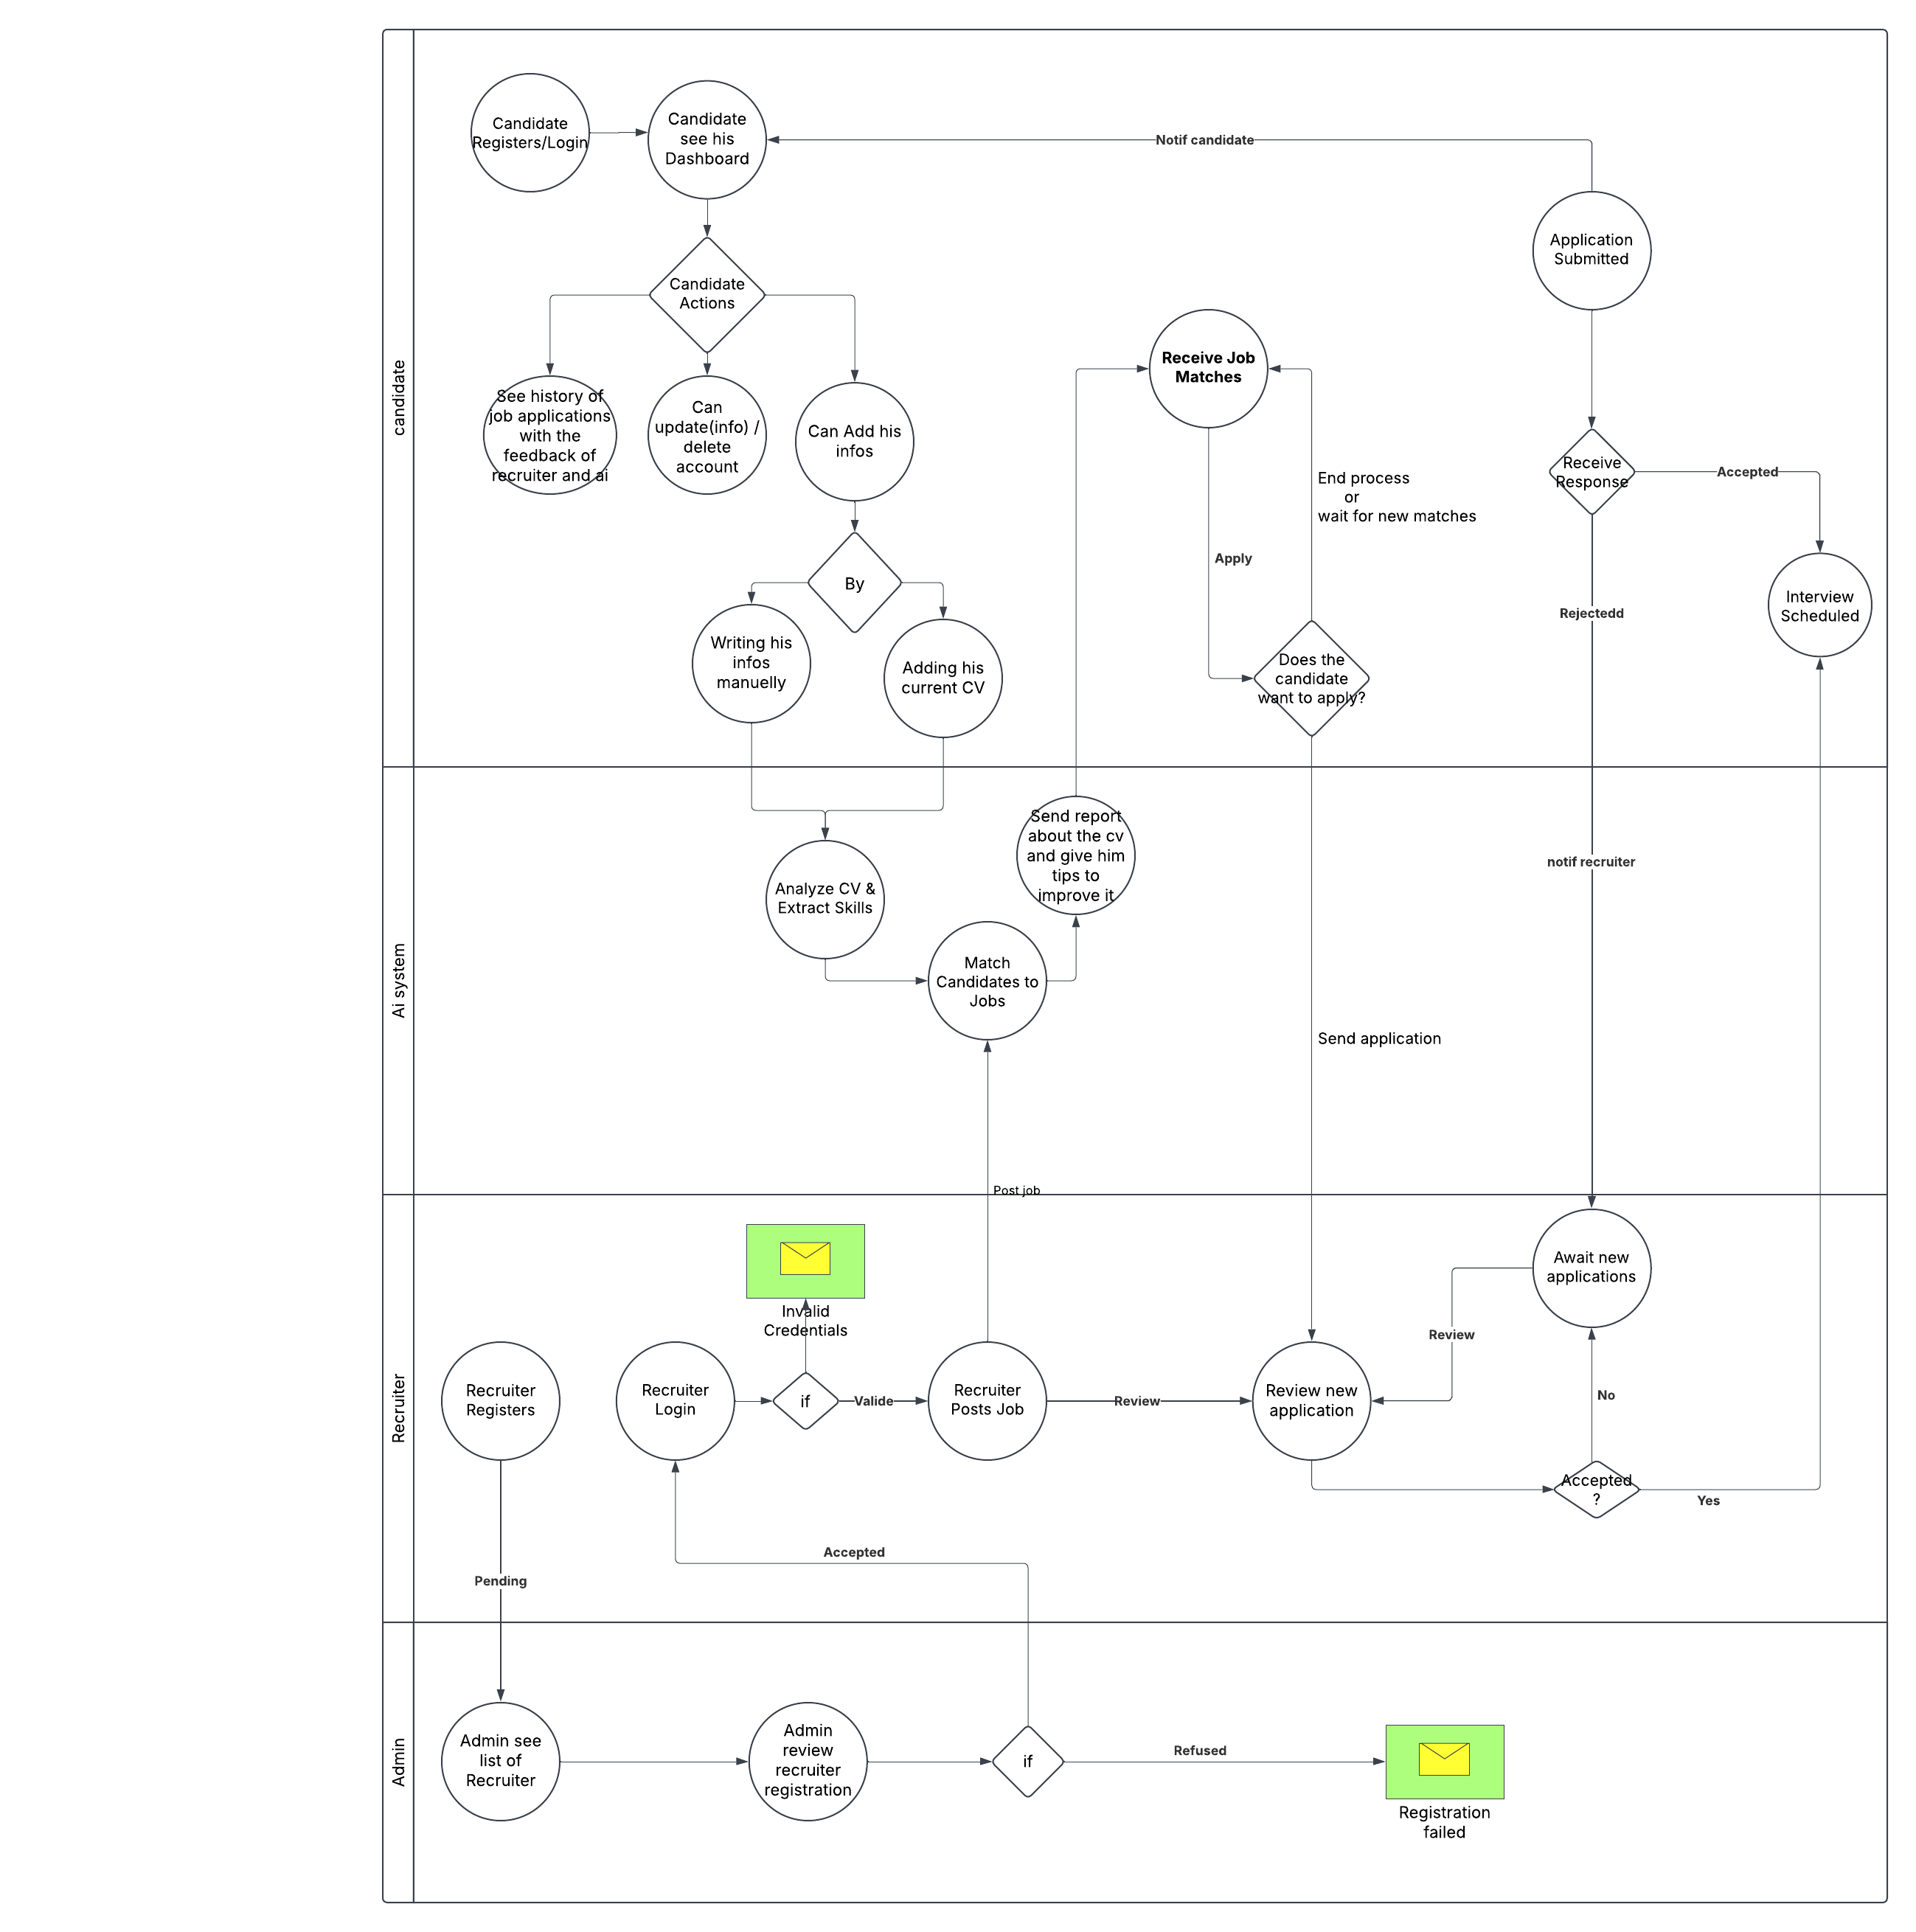
\includegraphics[width=0.9\textwidth]{Diagrams/BPMN.png}
    \caption{Diagram d'ativité}
    \label{fig:Diagram d'ativité}
\end{figure}
\newpage
\section{Conclusion}

Dans ce chapitre, nous avons discut'e des acteurs, des exigences fonctionnelles et non fonctionnelles de l'application. Nous avons ensuite expliqu'e la diff'erence entre les classes du diagramme et pr'epar'e le backlog de notre application. Enfin, nous avons pr'esent'e l’environnement de travail et l’architecture du projet.

Dans le prochain chapitre, nous expliquerons le processus et l’avancement du second sprint.


\section{Burndown Chart du Sprint 1}

Le sprint 1 \'etait principalement ax\'e sur la d\'ecouverte des frameworks, la probl\'ematique et la mise en place des routines avec la soci\'et\'e d’h\'ebrgement.


\stepcounter{mainsection} 
\setcounter{section}{0} 
\newpage
\section*{Chapitre 3 :}
\section*{ Sprint 2}
\subsubsection*{ Espace Candidate}
\section{Introduction}
Décris ici les fonctionnalités développées dans le premier sprint.

\section{ Product Backlog of sprint 2}
\begin{figure}[h]
    \centering
    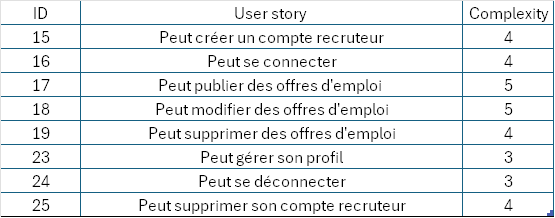
\includegraphics[width=0.8\textwidth]{Diagrams/backlog_de_produit_sprint1.png}
    \caption{Backlog du sprint}
    \label{fig:Backlog du sprint}
\end{figure}
\section{Conception}
Recherche de diagram pour react et express
\newpage
\section{Realisation}
    Dans cette section, nous présenterons le travail accompli durant ce sprint, illustré par des captures d'écran des tâches finalisées.

\subsection{Interface de registrement}
sign up 
\begin{figure}[h]
    \centering
    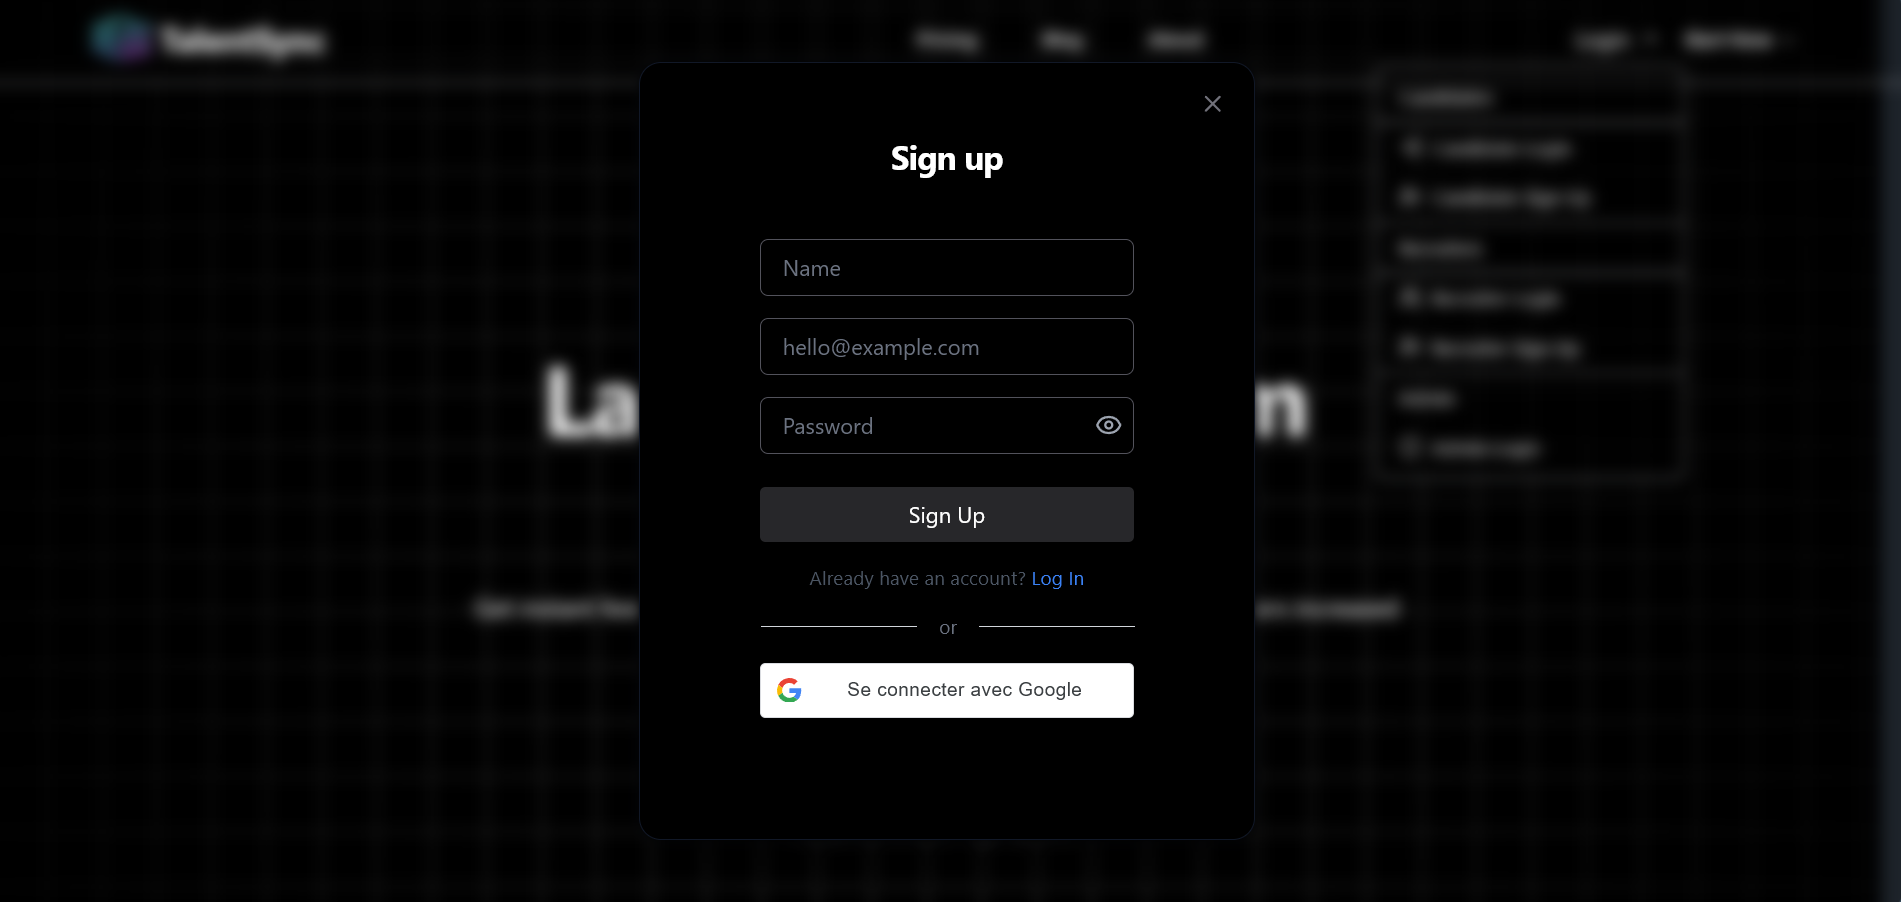
\includegraphics[width=1\textwidth]{Interfaces/Signup_candidate.png}
    \caption{Signup interface}
    \label{fig:Signup interface}
\end{figure}
\newpage
\subsection{Interface de registrement}
sign up 
\begin{figure}[h]
    \centering
    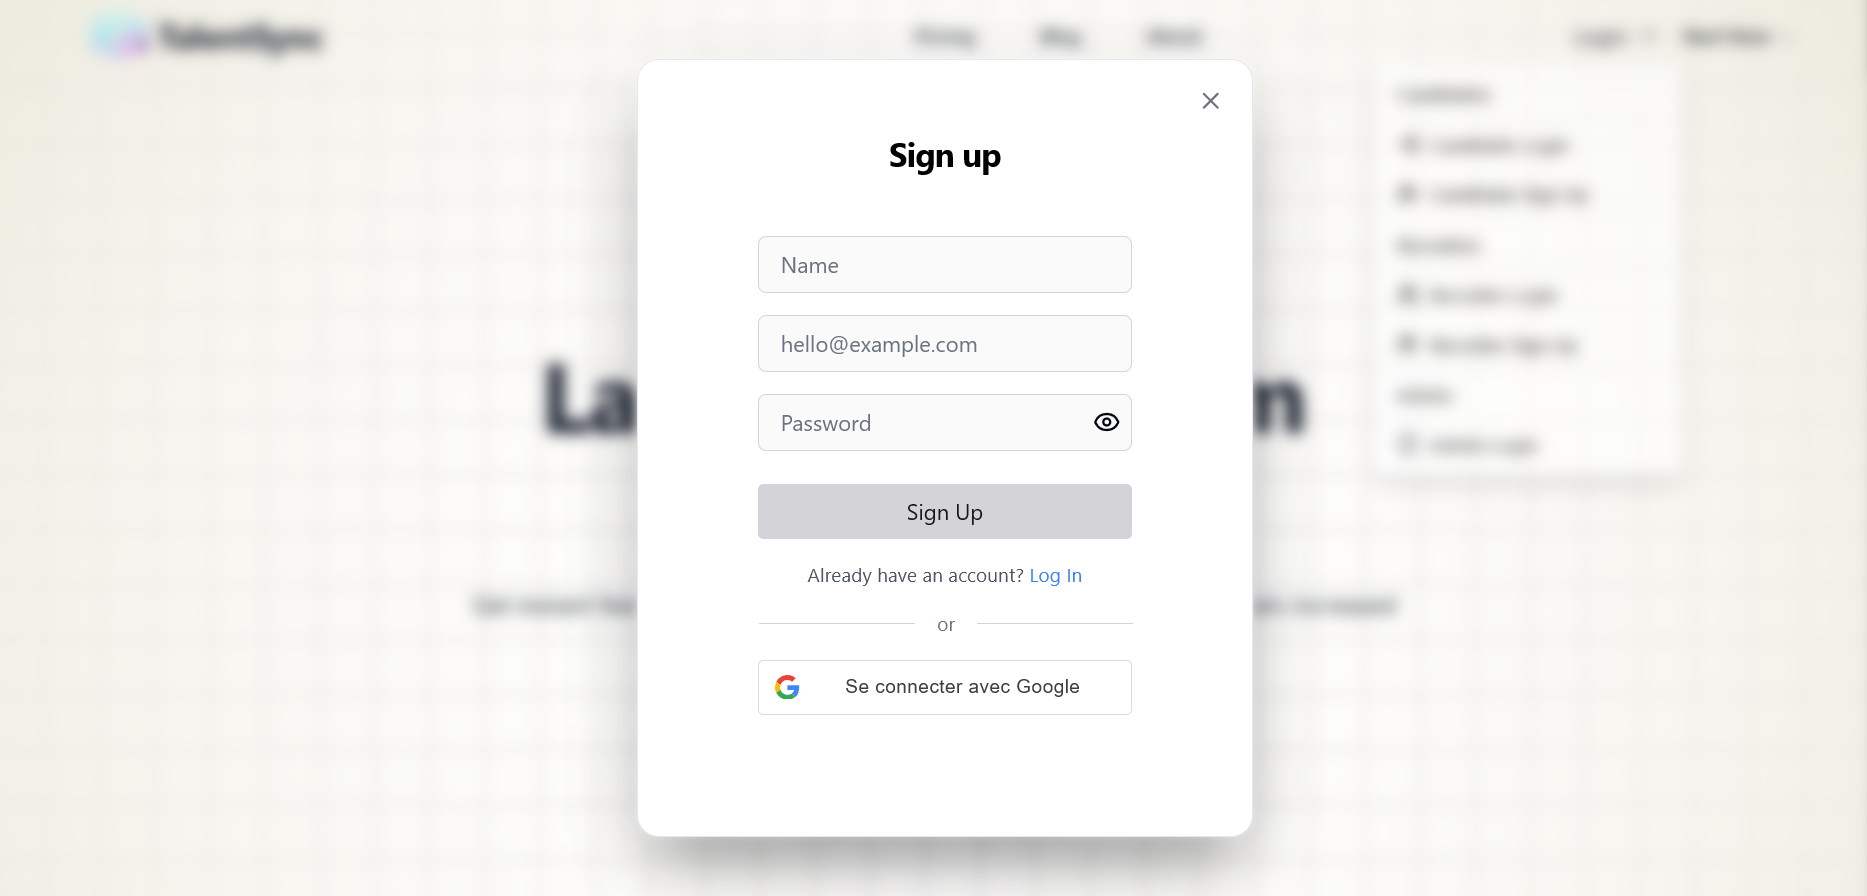
\includegraphics[width=1\textwidth]{Interfaces/Signup_candidate_w.png}
    \caption{Signup interface w}
    \label{fig:Signup interface w}
\end{figure}


\newpage
\subsection{Interface de login}
Login
\begin{figure}[h]
    \centering
    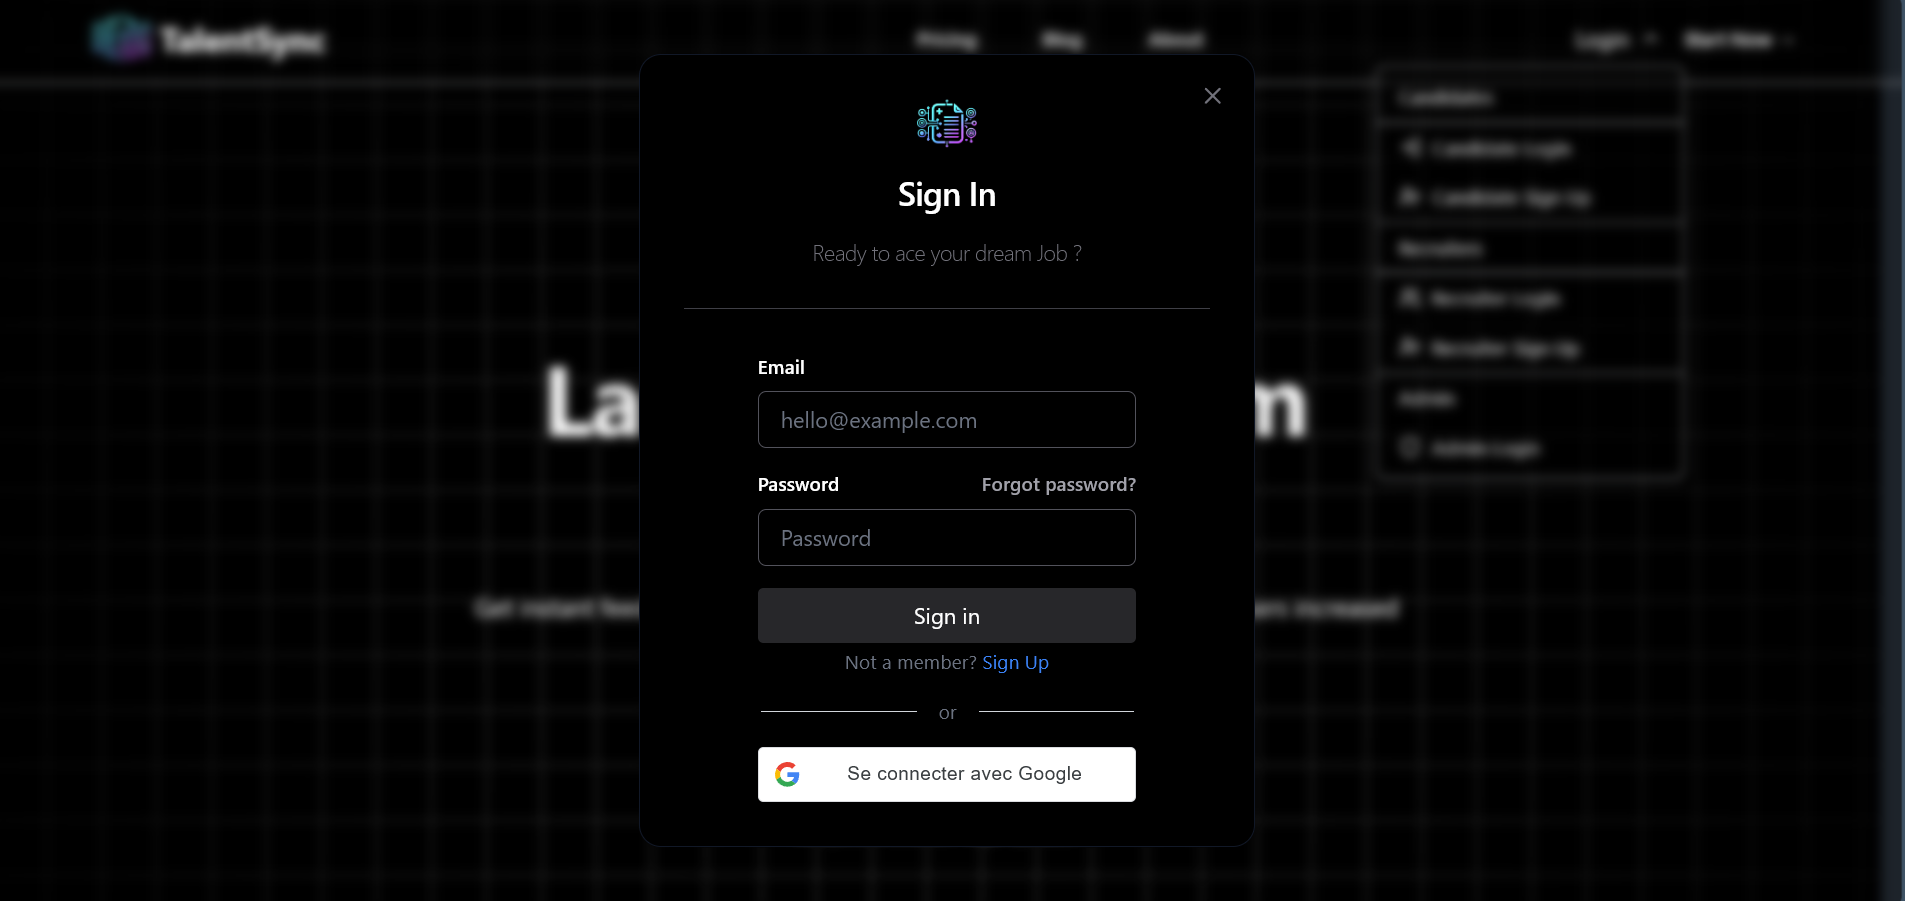
\includegraphics[width=1\textwidth]{Interfaces/Login_candidate.png}
    \caption{Login interface}
    \label{fig:Login interface}
\end{figure}

\newpage
\subsection{Interface de login}
Login
\begin{figure}[h]
    \centering
    \includegraphics[width=1\textwidth]{Interfaces/Login_candidate_W.png}
    \caption{ interface white mode}
    \label{fig: interface white}
\end{figure}



\newpage
\section*{Chapitre 3 : Sprint 3}
\subsection*{Espace Recruiter}
Décris ici les évolutions du projet.

\newpage
\section*{Chapitre 4 : Sprint 3}
\subsection*{PARTIE AI }
Explique les tests effectués, les corrections apportées et la conclusion du projet.



\end{document}